\documentclass[a4paper,12pt]{article}
\usepackage[top=2cm, bottom=2cm, left=2.5cm, right=2.5cm]{geometry} %margens
\usepackage[utf8]{inputenc}%assim aparecem os acentos
\usepackage{amsmath}
\usepackage{graphicx}
\usepackage[portuguese]{babel} % Para termos legendas em português 
% \title{Meu artigo} 
\usepackage{caption}
\usepackage{setspace}
\usepackage{hyperref}

\begin{document}
% \maketitle

\begin{center}
    Modelo de Suspensão de um Automóvel

\end{center}


\begin{figure}[h]

    \centering % para centralizarmos a figura
    \caption{Suspensão Simplificada de um Automóvel}
    \centering
    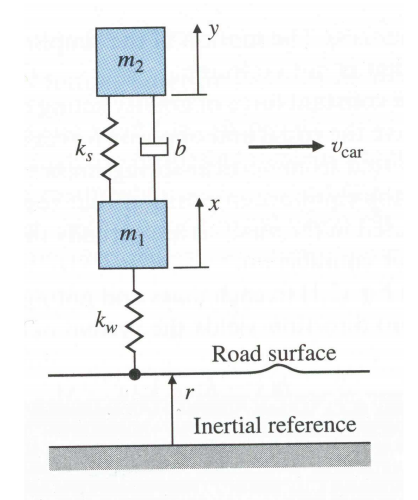
\includegraphics[width=9cm]{Imagens/img1.png} % leia abaixo
    \caption*{Fonte:VON ZUBEN}
    %\label{fig:test}
    \label{figura:susp_simplificada}
\end{figure}

%Na Fig. \ref{figura:susp_simplificada}, vemos que ...

\textbf{1.} Valores de $x$ e $y$ diferente de zero retratam deslocamentos das massas $m_1$ e $m_2$,
respectivamente, da condição de equilíbrio.

\textbf{2.} A mola com coeficiente $k_w$ compressividade do pneu, a qual vai ser proporcional
à diferença entre a posição da roda e o nível da superfície.

\textbf{3.} O deslocamento e a velocidade de deslocamento percebidas, respectivamente, pela
mola com coeficiente $k_s$ e amortecedor com coeficiente b são medidas relativas ao
deslocamento entre as duas massas (há acoplamento físico), dadas por:
%v$\Bigg\lbrace \dfrac{2}{4}$


$$
    \begin{cases}

        \mbox{deslocamento} = y - x \\

        \mbox{velocidade } \mbox{de } \mbox{deslocamento}= \dot{y} - \dot{x}
    \end{cases}
$$


\textbf{4.} Como os diagramas de corpo livre abaixo retratam forças agindo nas massas $m1$ e
$m2$ a partir de uma condição de equilíbrio, não são incluídas as forças de gravidade
$m_1g$ e $m_2g$, pois estas são supostas já anuladas por um deslocamento constante nas
molas com coeficientes $k_s$ e $k_w$. Estes deslocamentos são dados por:

$$
    \begin{cases}

        deslocamento_s = & \dfrac{m_2g}{k_s}       \\

        deslocamento_w = & \dfrac{(m_1+m_2)g}{k_w}
    \end{cases}
$$

\textbf{5.} Os diagramas de corpo livre a seguir não incluem a força de reação à aceleração
de massa, dada pela segunda lei de Newton.

\begin{figure}[ht]

    \centering % para centralizarmos a figura
    \caption{Diagramas de Corpo Livre}
    \centering
    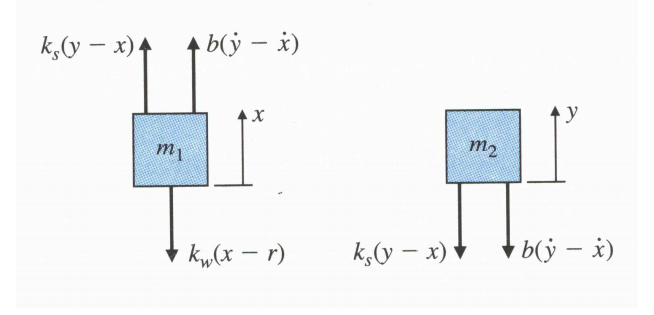
\includegraphics[width=15cm]{Imagens/img2.png} % leia abaixo
    \caption*{Fonte:VON ZUBEN}
    %\label{fig:test}
    \label{figura:dcl}

\end{figure}





$$
    \mbox{Equações } \mbox{do } \mbox{movimento:}
    \begin{cases}

        m_1\ddot{x} - b(\dot{y}-\dot{x})-k_s(y-x)+k_w(x-r) = 0 \\

        m_2\ddot{x} + b(\dot{y}-\dot{x})-k_s(y-x) = 0
    \end{cases}
$$


$$
\mbox{Após } \mbox{manipulação } \mbox{algébrica:}
\begin{cases}

    \ddot{x} + \dfrac{b}{m_1}(\dot{x}-\dot{y})+\dfrac{k_s}{m_1}(x-y)+\dfrac{k_w}{m_1}x = \dfrac{k_w}{m_1}r \\

    \ddot{y} + \dfrac{b}{m_2}(\dot{y}-\dot{x})+\dfrac{k_s}{m_2}(y-x) = 0
\end{cases}
$$


\textbf{Referências:}

\begin{enumerate}
    \item VON ZUBEN, Fernando J. \textbf{Modelagem de Sistemas Dinâmicos Contínuos no Tempo}.
    Disponível em: \url{ftp://ftp.dca.fee.unicamp.br/pub/docs/vonzuben/ea616_1s10/notas_de_aula/topico3_EA616_1s2010.pdf}.Acesso em: 09/11/2020.
\end{enumerate}



\end{document}

